\section{Apache Hadoop}
\label{sec:hadoop}

\textbf{Apache\texttrademark Hadoop\textregistered}\footnote{\url{https://hadoop.apache.org/}} ist ein Open"=Source"=Software"=Projekt, welches die Verarbeitung von großen Datenmengen auf einem verteilten System ermöglicht.
Hadoop wird von der \emph{Apache Foundation} entwickelt und stellt und enthält verschiedene vollständig skalierbare Komponenten.
Es ist daher möglich, ein Hadoop"=Cluster auf nur einem einzelnen PC, aber auch verteilt auf zahlreichen Servern auszuführen.
Hadoop ermöglicht es dadurch, sehr einfach \glspl{Anwendung} auszuführen, um große Datenmengen zu verarbeiten.
Die für das Cluster, und damit den Anwendungen, verfügbaren Ressourcen beschränken sich lediglich auf die Summe der verfügbaren Ressourcen aller Hosts, auf denen das Cluster ausgeführt wird.

Hadoop besteht aus folgenden Kernmodulen \cite{HadoopHomePage}:

\begin{description}
	\item[Hadoop Common] \hfill \\
        Gemeinsam genutzte Kernkomponenten
	\item[Hadoop \acrshort{YARN} (\acrlong{YARN}\glsunset{YARN})] \hfill \\
        Framework zur Verteilung und Ausführung von \glspl{Anwendung} und das dazugehörige Ressourcen"=Management
	\item[\acrlong{HDFS}] \hfill \\
        Kurz \acrshort{HDFS}\glsunset{HDFS}, verteiltes Dateisystem
	\item[Hadoop \acrlong{MR}] \hfill \\
        Kurz \acrshort{MR}\glsunset{MR}, Implementierung des \gls{MR}"=Ansatzes zum Verarbeiten von großen Datenmengen, nutzt \gls{YARN} zur Ausführung der Anwendungen
\end{description}

Aufgrund seiner Verbreitung stellt Hadoop eine der wichtigsten Implementierungen des \gls{MR}"=Ansatzes dar \cite{PoweredByHadoop}.
Die Eingabe"= und Ausgabedaten sind hierbei als \emph{Key"=Value}"=Paare definiert, die mithilfe des \gls{MR}"=Frameworks verarbeitet werden.
Hierbei werden zunächst die eingelesenen Eingabedaten in kleine und dadurch einfach zu verarbeitende Datenmengen aufgeteilt.
Die geteilten Daten werden dann in mehreren, parallel ausgeführten Map"=Tasks verarbeitet und zwischengespeichert.
Die zwischengespeicherten Daten werden anschließend von einem oder mehreren Reduce"=Tasks zusammengeführt und in die Ausgabedateien geschrieben.
Das Framework ist hierbei sehr Fehlertolerant, da ein fehlerhafter Task jederzeit neu gestartet werden kann \cite{Dean2004,Dean2010}.
Zur Speicherung der Ein-, Zwischen- und Ausgabedaten wird im Falle von Hadoop das \gls{HDFS} genutzt \cite{HadoopMapRedTutorial271}.
Für weitere Details zum \gls{MR}"=Framework sei hier auf \cite{Dean2004} und \cite{Dean2010} verwiesen, eine ausführliche Betrachtung des \gls{MR}"=Frameworks mit Vorteilen und Problemen lässt sich in \cite{Lee2012} finden.

Da das \gls{MR}"=Framework bzw. seine Implementierung in Hadoop nicht perfekt ist und in der Praxis zum Teil auch zweckentfremdet wurde, wurde in \cite{Vavilapalli2013} das \textbf{\gls{YARN}}"=Framework vorgestellt.
Die Kernidee ist hierbei die Trennung von Ressourcenmanagement und Scheduling vom eigentlichen Programm.
In diesem Kontext bildet der \gls{MR}"=Ansatz eine mögliche Anwendung, die mithilfe des \gls{YARN}"=Frameworks ausgeführt wird \cite{Vavilapalli2013}.

Ein Hadoop"=Cluster mit dem \gls{YARN}"=Framework besteht aus zwei wesentlichen Komponenten, dem \emph{Controller} mit \gls{RM} und den angeschlossenen \emph{Nodes}:

\begin{figure}[h]
    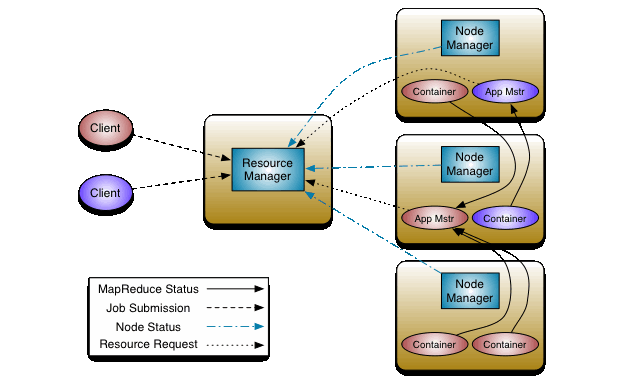
\includegraphics{./resources/yarn_architecture.png}
    \caption[Architektur des YARN"=Frameworks]
    {Architektur des \gls{YARN}"=Frameworks (entnommen aus \cite{HadoopYarnArch271})}
    \label{fig:yarnarch}
\end{figure}

Der \gls{RM} dient hierbei als \emph{Load"=Balancer} für das gesamte Cluster und besteht aus dem \gls{AM} und dem \emph{Scheduler}, die eigentliche Ausführung der \glspl{Anwendung} findet auf den Nodes statt.
Der \gls{AM} ist für die Annahme und Ausführung von einzelnen \glspl{Anwendung} zuständig, denen der Scheduler die dafür notwendigen Ressourcen im Cluster zuteilt.
Jeder Node besitzt einen \gls{NM}, der für die Überwachung der Ressourcen auf dem jeweiligen Node sowie der auf dem Node ausgeführten Anwendungs"=Container zuständig ist und diese Daten dem \gls{RM} übermittelt.

Jede \gls{YARN}\gls{Anwendung} bzw. Job besteht aus einer oder mehreren Ausführungsinstanzen, genannt Attempts.
Jeder \gls{Attempt} besitzt einen eigenen \gls{AppMstr}, welcher das Monitoring der \gls{Anwendung} und die Kommunikation mit dem \gls{RM} und \gls{NM} übernimmt und die dafür benötigten Informationen bereitstellt \cite{HadoopYarnArch271}.
Die eigentliche Ausführung einer \gls{Anwendung} findet in den bereits erwähnten \emph{Containern} statt, die jeweils einem \gls{Attempt} zugeordnet sind.
Container können auf einem beliebigen Node ausgeführt werden und repräsentieren die Ausführung eines Tasks innerhalb der Anwendung.

Zu erwähnen ist hier zudem, dass die Kommunikation zwischen den einzelnen Komponenten nicht in allen Fällen in Echtzeit statt findet.
Vor allem das Prüfen des generellen Node"=Zustandes durch den \gls{RM} wird bei einer Standard"=Konfiguration in periodischen Abständen von jeweils mehreren Minuten durchgeführt.
Sollte der \gls{NM} bei solchen Status"=Abfragen zunächst nicht reagieren, wird mehrere Minuten gewartet, bis der Node als defekt erkannt wird.
Ähnlich verhält es sich bei Zustandsabfragen an den \gls{AppMstr} \cite{HadoopYarnConfig271}.

Ein weiterer Bestandteil von Hadoop bzw. \gls{YARN} ist der \gls{TLS}.
Er ist speziell dafür entwickelt, die Metadaten und Logs der \gls{YARN}\gls{Anwendung}en zu speichern und jederzeit, also als Anwendungshistorie, auszugeben \cite{HadoopYarnTlServer271}.

Zum Steuern des Clusters bzw. dem Monitoring der mithilfe von \gls{YARN} ausgeführten \glspl{Anwendung} stellt Hadoop drei Schnittstellen zur Verfügung.
Dies sind eine graphische Weboberfläche, was zugleich auch die wichtigste Schnittstelle darstellt, entsprechende Befehle für die \acrlong{CLI} (engl. \emph{Command-line interface}, kurz \acrshort{CLI})\glsunset{CLI}, sowie eine \gls{REST}"=API.
Während sich die Weboberfläche zur menschlichen Interaktion oder zum Finden von Fehlern eignet, dienen die \gls{CLI}"=Befehle vor allem zum Steuern des Clusters und die \gls{REST}"=API zur automatisierten Rückgabe der Daten des Clusters zur Nutzung in anderen Programmen \cite{HadoopClusterSetup271,HadoopYarnCmds271,HadoopRmApi271,HadoopNmApi271}.

Das \textbf{\gls{HDFS}} basiert auf einer ähnlichen Architektur wie \gls{YARN} und besitzt ebenfalls einen Controller und mehrere Nodes:

\begin{figure}[h]
    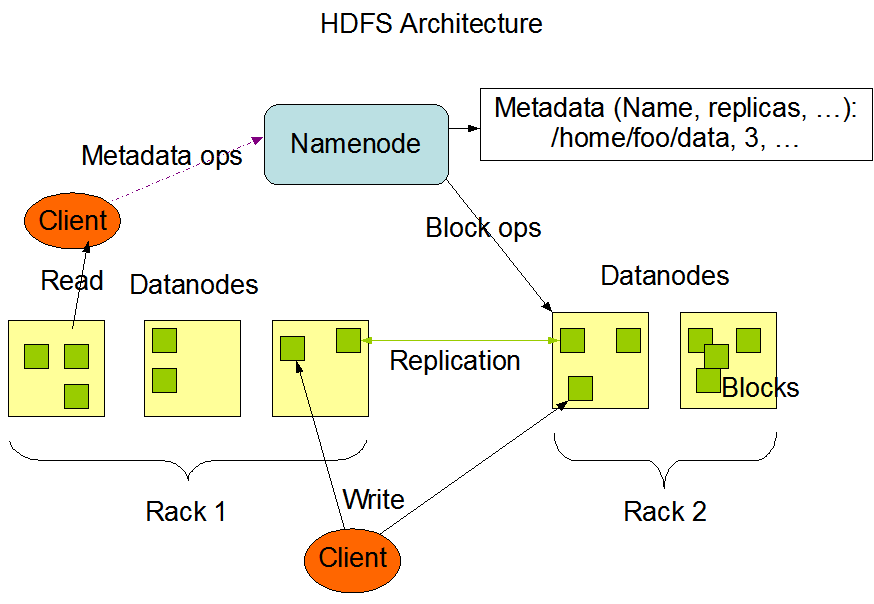
\includegraphics{./resources/hdfsarchitecture.png}
    \caption[Architektur des HDFS]
    {Architektur des \acrshort{HDFS} (entnommen aus \cite{HadoopHdfsDesc271})}
    \label{fig:hdfsarch}
\end{figure}

Der \emph{NameNode} dient als Controller für die Verwaltung des Dateisystems und reguliert den Zugriff auf die darauf gespeicherten Daten.
Unterstützt wird der NameNode vom \emph{Secondary NameNode}, der Teile der internen Datenverwaltung des \gls{HDFS} durchführt \cite{HadoopHdfsGuide271}.
Die Daten selbst werden in mehreren Blöcke aufgeteilt auf den \emph{DataNodes} gespeichert.
Um den Zugriff auf die Daten im Falle eines Node"=Ausfalls zu gewährleisten, wird jeder Block auf anderen Nodes repliziert.
Dateioperationen (wie Öffnen oder Schließen) werden direkt auf den DataNodes ausgeführt.
Sie sind darüber hinaus auch dafür verantwortlich, dass die gespeicherten Daten gelesen und beschrieben werden können \cite{Shvachko2010,HadoopHdfsDesc271}.

Das Überprüfen der DataNodes durch den NameNode erfolgt genauso wie bei den entsprechenden \gls{YARN}"=Komponenten periodisch im Abstand von mehreren Minuten.
Auch hier dauert es bei einer Standard"=Konfiguration daher mehrere Minuten, bis erkannt wird, wenn ein DataNode nicht mehr verfügbar ist \cite{HadoopHdfsConfig271}.
